\chapter{Strumenti e tecnologie}
\label{cap:strumenti-tecnologie}

\intro{L'obiettivo principale di questo capitolo è l'illustrazione delle tecnologiene degli strumenti ausiliari utilizzati per raggiungere lo scopo finale del progetto}\\

\section{Strumenti}
\label{sec:strumenti}
Gli strumenti di supporto adoperati per il progetto sono elencati nella lista seguente.

\begin{itemize}
    \item Visual Studio Code (Fig.~\ref{fig:logo-vscode}): è un ambiente di sviluppo integrato, disponibile per Linux, macOS e Windows. 
    È un'applicazione che supporta la maggior parte dei linguaggi di programmazione ed è quindi molto vantaggiosa per lavorare ad un progetto multi-linguaggio senza dover cambiare ambiente.
    Un'altra delle funzionalità principali è la fornitura di numerose estensioni che semplificano il processo di scrittura e verifica del codice.

    \begin{figure}[!h] 
        \centering 
        
\includegraphics[width=0.4\columnwidth]{tecnologie/visual-studio-logo.png} 
        \caption{Logo di Visual Studio Code}
        \label{fig:logo-vscode}
      \end{figure}

\newpage

    \item PhpMyAdmin (Fig.~\ref{fig:logo-phpmyadmin}): è una web-app scritta utilizzando il linguaggio di programmazione PHP, che offre la capacità di gestione di un database MySQL attraverso un browser qualsiasi. Consente la creazione di tabelle, l'inserimento, la modifica e l'interrogazione dei dati.
    Fornisce un'interfaccia grafica per la visione d'insieme e per le operazioni amministrative.

    \begin{figure}[!h] 
        \centering 
        
\includegraphics[width=0.4\columnwidth]{tecnologie/phpmyadmin-logo.png} 
        \caption{Logo di phpMyAdmin}
        \label{fig:logo-phpmyadmin}
      \end{figure}

    
    \item Remote Ripple (Fig.~\ref{fig:logo-remoteripple}): è un software per l'accesso remoto, che viene utilizzato dallo studente per avviare i programmi presenti nel server aziendale.
    
    \begin{figure}[!h] 
        \centering 
        
\includegraphics[width=0.3\columnwidth]{tecnologie/remote-ripple-logo.png} 
        \caption{Logo di Remote Ripple}
        \label{fig:logo-remoteripple}
      \end{figure}

\end{itemize}

\newpage

\section{Tecnologie}
\label{sec:tecnologie-strumenti}

Nelle sezioni seguenti viene data una spiegazione di tutte le tecnologie utilizzate.

\subsection{Python}

\subsubsection{Versione: 3.9.0}
Python (Fig.~\ref{fig:logo-python}) è un linguaggio di programmazione ampiamente utilizzato in settori come il data mining e l'intelligenza artificiale. 
Offre solide basi per l'integrazione con disparati linguaggi, ma il vantaggio più di risalto è la presenza di numerose librerie che aiutano lo sviluppatore a velocizzare il processo di codifica; in particolare sono state utilizzate le seguenti librerie:

\subsubsection{Tensorflow-gpu 2.10.1}
TensorFlow è una framework utilizzato per il machine-learning, su di esso si basa tutta la struttura del progetto.\\
L'unità di base del framework è il tensore, ossia un vettore di n dimensioni, tutte le operazioni possibili vengono eseguite su elementi appartenenti a questo tipo.
Inoltre contiene modelli pre-addestrati molto utili per eseguire determinate operazioni in maniera più rapida. 
Viene utilizzata la versione 2.10 perché è l'ultima ad avere il supporto per GPU su sistema operativo Windows.

\subsubsection{Keras 2.10.0}
Keras è un API sviluppata per rendere la codifica di IA più semplice per la comprensione umana. 
Minimizza le azioni richieste all'utente per i casi d'uso più comuni, rendendo l'utilizzo di framework come JAX, TensorFlow e PyTorch più user-friendly.

\subsubsection{Scikit-Learn 1.5.2}
Scikit-learn è una libreria che offre semplici tool utili per la classificazione, la regressione, il clustering, eccetera.

\subsubsection{Matplotlib 3.9.2}
Matplotlib è una libreria che viene utilizzata per la stampa dei grafici ottenuti durante le varie compilazioni. 

\subsubsection{Numpy 1.26.4}
NumPY è il pacchetto che si occupa della gestione di array multi dimensionali fornendo anche un'ampia gamma di funzioni matematiche da applicare agli stessi.

\subsubsection{OpenCV-python 4.10.0}
OpenCV è una libreria utilizzata per sviluppare applicazioni di tipo computer vision. Nell'ambito del progetto il suo scopo primario è l'elaborazione delle immagini per adattarle all'utilizzo da parte delle IA. 

\subsubsection{Pyppeteer 2.0.0}
Pyppeteer è una libreria di automazione per browser basati su chromium.

\begin{figure}[!h] 
  \centering 
  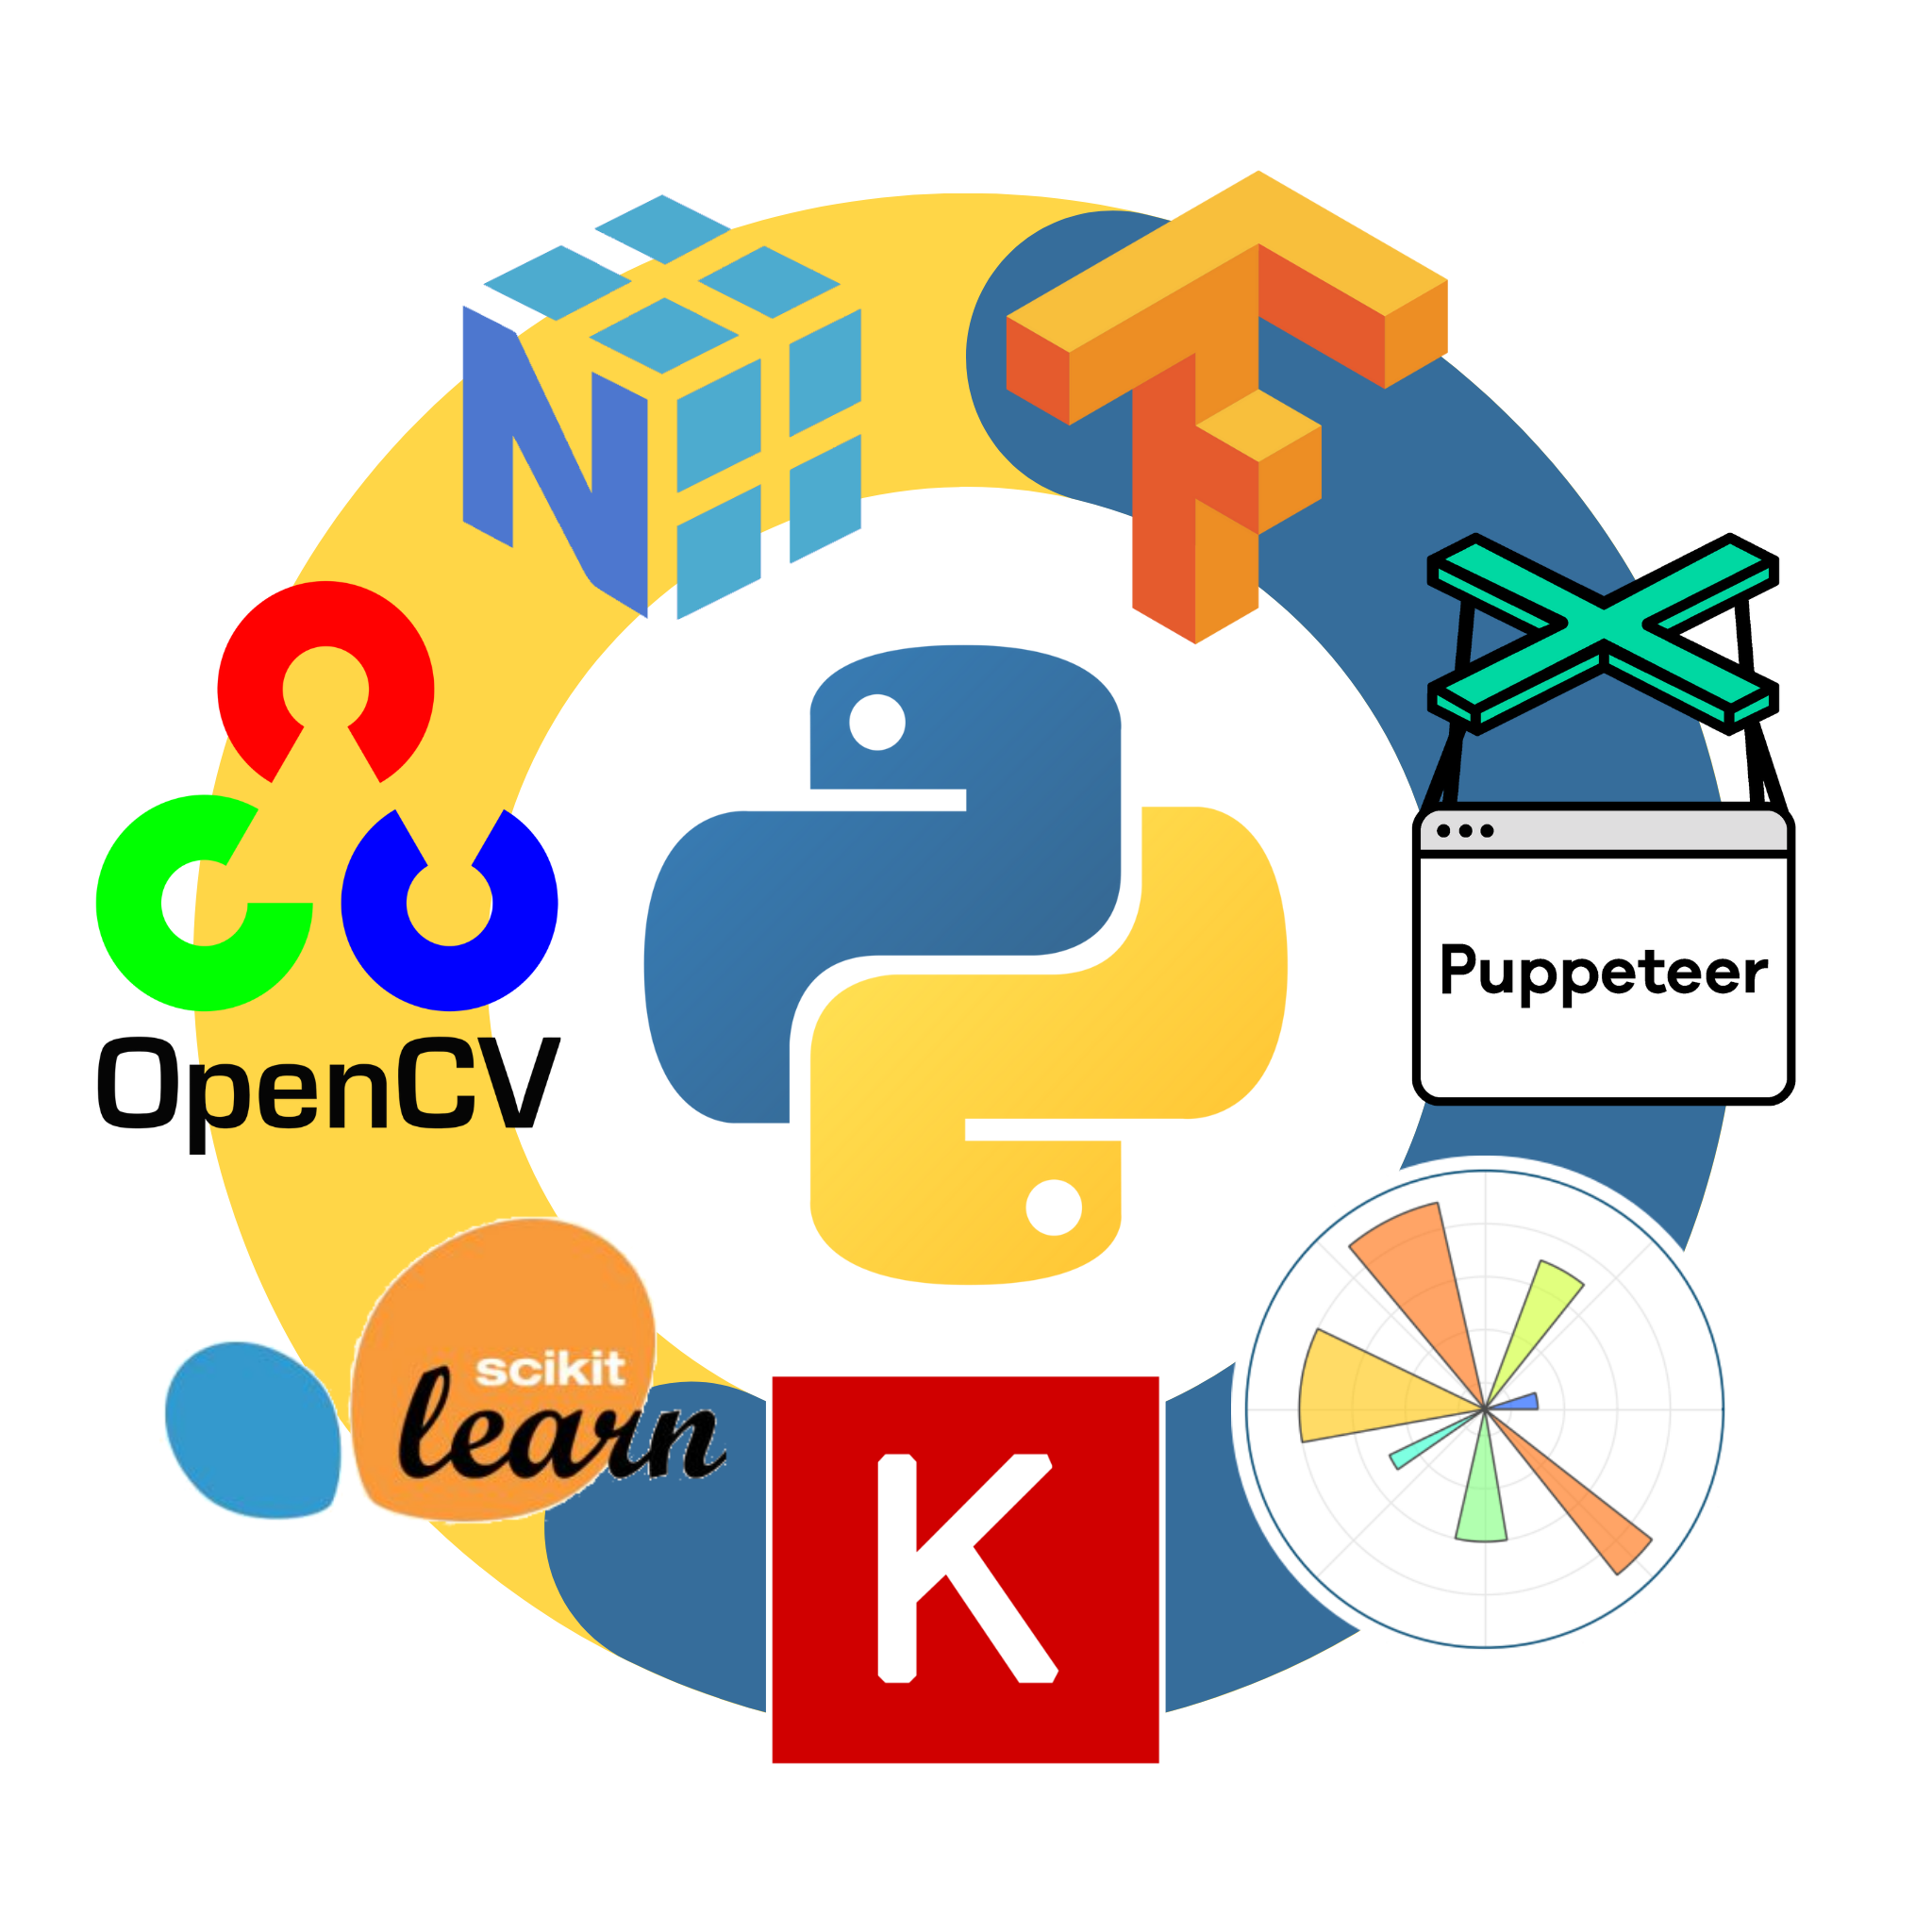
\includegraphics[width=0.8\columnwidth]{tecnologie/python-librerie.png} 
  \caption{Python e librerie utilizzate}
  \label{fig:logo-python}
\end{figure}



\subsection{CUDA}
\subsubsection{Versione: 11.2}
Descrizione Tecnologia 1

\subsection{Docker}
\subsubsection{Versione: 27.2.0}
Descrizione Tecnologia 2

\subsection{DDEV}
\subsubsection{Versione: 1.23.2}
Descrizione Tecnologia 3

\subsection{WSL}
\subsubsection{Versione: 2.3.24.0}
Descrizione Tecnologia 4

\subsection{\label{tec:Laravel}Laravel}
\subsubsection{Versione: 11.29.0}
Descrizione Tecnologia 5

\subsection{\label{tec:Filament}Filament}
\subsubsection{Versione: 3.2.121}
Descrizione Tecnologia 6

\subsection{MySQL}
\subsubsection{Versione: 8.0.36}
Descrizione Tecnologia 7

%AGGIUNGERE DA QUALCHE PARTE LE DIPENDENZE TRA LIBRERIE E VERSIONI
\section{Ciclo di vita del software}
\label{sec:ciclo-vita-software}

\section{Progettazione}
\label{sec:progettazione}

\subsubsection{Namespace 1} %**************************
Descrizione namespace 1.

\begin{namespacedesc}
    \classdesc{Classe 1}{Descrizione classe 1}
    \classdesc{Classe 2}{Descrizione classe 2}
\end{namespacedesc}


\section{Design Pattern utilizzati}

\section{Codifica}
